%!TEX root = minta_dolgozat.tex
%%%%%%%%%%%%%%%%%%%%%%%%%%%%%%%%%%%%%%%%%%%%%%%%%%%%%%%%%%%%%%%%%%%%%%%
\chapter{Eredmények és következtetések}\label{ch:eredmenyek}
%%%%%%%%%%%%%%%%%%%%%%%%%%%%%%%%%%%%%%%%%%%%%%%%%%%%%%%%%%%%%%%%%%%%%%%

A háló teszteléséhez a tesztelési adatokból kivágott forgalmi táblákat használtam. 

Különböző paraméterekre (rétegek száma, rejtett réteg/rétegek mérete, batch méret, tanulási ráta) folytattam tesztelést az ideális körülmények megtalálása érdekében. Eleinte nem a teljes adathalmazra, hanem csak pár osztályra futtattam, a gyors eredmény érdekében. Ezek a tesztek gyorsan lefutottak és viszonylagos eredményt adtak a hálóról.

Amikor kis adathalmazzal teszteltem, kevés osztállyal, azt tapasztaltam, hogy ha az osztályok olyan táblákat tartalmaztak amik jelentősen különböznek egymástól, akkor 100\%-ban felismeri a tesztadatokat. Ilyen osztályokra példa a STOP tábla és a 30-as sebességkorlátozó tábla. Abban az esetben, ha az osztályokba tartozó táblák hasonlítanak egymásra, mint például a 30-as és 50-es sebességkorlátozó tábla, a felismert táblák száma lecsökken, kb. 85\%-ra.

\section{Rétegek számának meghatározása}

A rendszer a legjobb eredményt akkor adta, ha nem volt jelen rejtett réteg. Az által, hogy nem volt rejtett réteg a számítások egyszerűsödtek és a folyamat felgyorsult.

Abban az esetben, ha egy rejtett réteg volt, a tanulás kb. 100 ciklus után kezdődött el. A tanulási folyamat lassú volt és a végeredmény nem mutatott jobb eredményt mint amikor hiányzott a rejtett réteg.

Az elkövetkezendő teszteredmények olyan rendszerben készültek, ahol nem volt jelen rejtett réteg.

\section{Tanulási ráta meghatározása}

A tanulási ráta behatárolására először három, négy osztályra futtattam teszteket. Ez által gyorsan kaptam egy viszonyítási pontot, amit majd alkalmazni tudtam a több osztályra történő futáskor.

Elsőnek 1-es tanulási rátával próbálkoztam. Az eredmények elég pozitívak voltak, a \ref{fig:learningrate1} ábrán látható a helyesen kategorizált képek száma minden ciklusban.

\begin{figure}
\centering

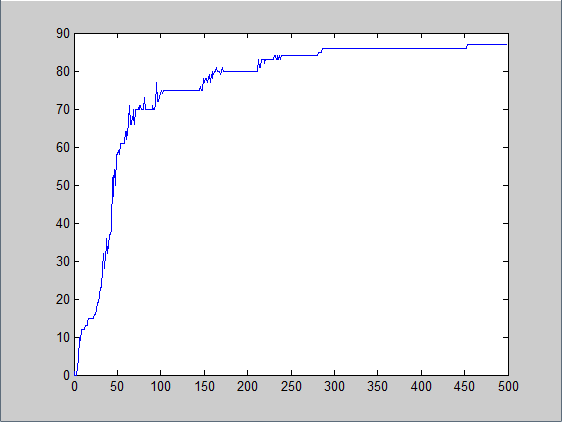
\includegraphics[scale=0.5]{images/Teszt2}
\caption{1-es tanulási ráta}

\label{fig:learningrate1}
\end{figure}

Ezek után a tanulási ráta növelésével próbálkoztam. Habár a helyesen kategorizált képek száma minimálisan csökkent, ebben az esetben a háló sokkal hamarabb kezdte megtanulni az osztályok jellemzőit. A \ref{fig:learningrate2} ábrán jól látszik, hogy sokkal meredekebb az elején, vagyis gyorsabban tanul az elején és utána normalizálódik. A maximum elérése után a kezdeti oszcilláció is megszűnik.

\begin{figure}
\centering

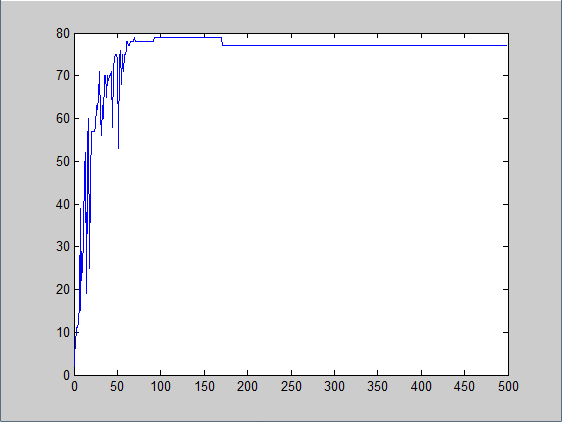
\includegraphics[scale=0.5]{images/Teszt3}
\caption{3-as tanulási ráta}

\label{fig:learningrate2}
\end{figure}

Végeztem teszteket más értékű tanulási rátával is, de ha nem változtattam nagy mértékben az értéket, akkor hasonló eredményt adtak. Ha túlságosan megnöveltem az értékét, az oszcilláció ami a \ref{fig:learningrate2} ábra elején látható megnőtt és nagy mértékben lecsökkent a felismert táblák száma. Ha túl kicsi értéket választottam, a tanulási folyamat nagyon lassan indult be. Ebből kiindulva a további tesztekhez a tanulási rátát háromnak választottam meg.

\section{Batch méretének meghatározása}

A batch méretének meghatározásához is több tesztet futtattam különböző értékekre. A behatárolást ebben az esetben is kis méretű adathalmazra végeztem.

A batch méretének változtatása nem volt nagy hatással a helyesen kategorizált képek számára. A  \ref{fig:batchsize1}, \ref{fig:batchsize2} és \ref{fig:batchsize3} ábrákon látható a 10-re, 20-ra, illetve 30-ra kapott eredmények. Nincs nagy különbség közöttük, de a 30-as értékre let legnagyobb a felismert táblák száma, ezért a továbbiakban ezzel az értékkel dolgoztam. Nagyobb mennyiségű tesztadatra megpróbáltam később a bath méretét 10-re állítani, de a tanulás jelentősen nehezebben indult be, ezért nem végeztem vele több tesztet. 

\begin{figure}
\centering

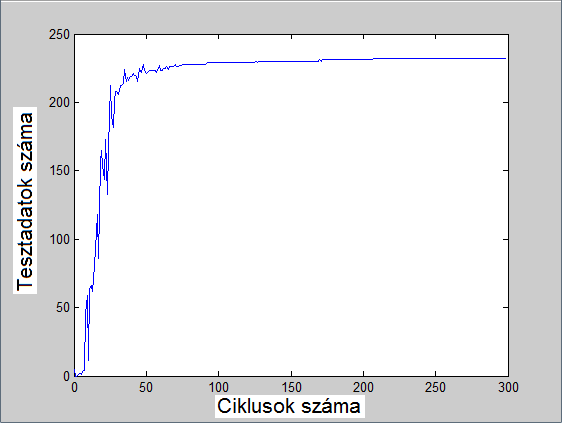
\includegraphics[scale=0.5]{images/Teszt7}
\caption{10-es bath méret eredményei}

\label{fig:batchsize1}
\end{figure}

\begin{figure}
\centering

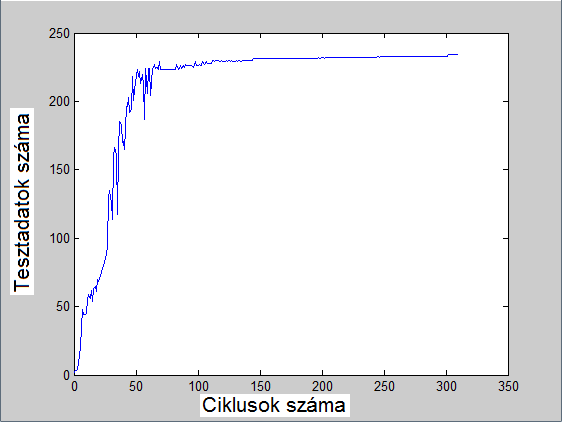
\includegraphics[scale=0.5]{images/Teszt8}
\caption{20-as bath méret eredményei}

\label{fig:batchsize2}
\end{figure}

\begin{figure}
\centering

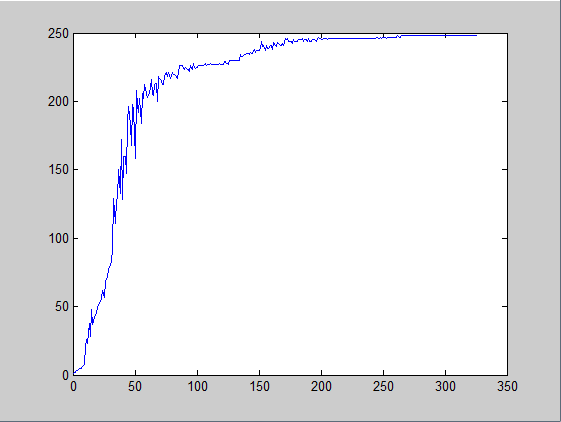
\includegraphics[scale=0.5]{images/Teszt9}
\caption{30-as bath méret eredményei}

\label{fig:batchsize3}
\end{figure}

\section{Ciklusok számának meghatározása}

A ciklusok száma a tanulási folyamatban nem játszik olyan fontos szerepet mint a tanulási ráta, viszont ha túl kicsinek választjuk meg a hálónak nincs elég ideje tanulni. A nagy ciklusszám nincs negatív hatással a felismert táblák számára, de feleslegesen növeli a futási időt. Miután a háló elérte azt a pontot, hogy nem képes tovább fejlődni, felesleges további ciklusokat futtatni. Lehetne egy olyan feltételt beiktatni, hogy ha egy bizonyos százalékban felismeri a háló a táblákat akkor állítsuk le a tanulást meg mielőtt az összes ciklust végrehajtanánk, de ha ezt a százalékot túl nagyra állítjuk és ez által elérhetetlenné válik, akkor felesleges, ha pedig túl kicsire, a futási időt ugyan lecsökkent, de a háló még képes lett volna tanulni tovább.

100 ciklus ez esetek többségében elégségesnek bizonyul, de néha 50 ciklus is ugyanazt eredményezte. 

